\documentclass[lettersize,journal]{IEEEtran}
\usepackage{amsmath,amsfonts}
\usepackage{algorithmic}
\usepackage{algorithm}
\usepackage{array}
\usepackage[caption=false,font=normalsize,labelfont=sf,textfont=sf]{subfig}
\usepackage{textcomp}
\usepackage{stfloats}
\usepackage{url}
\usepackage{verbatim}
\usepackage{graphicx}
\usepackage{cite}
\hyphenation{op-tical net-works semi-conduc-tor IEEE-Xplore}
% updated with editorial comments 8/9/2021

\begin{document}

\title{The Risks and Benefits of Social Media, and Its Place in Higher Education: a literature review}

\author{IEEE Publication Technology,~\IEEEmembership{Staff,~IEEE,}
        % <-this % stops a space
\thanks{This paper was produced by the IEEE Publication Technology Group. They are in Piscataway, NJ.}% <-this % stops a space
\thanks{Manuscript received April 19, 2021; revised August 16, 2021.}}

% The paper headers
\markboth{Journal of \LaTeX\ Class Files,~Vol.~14, No.~8, August~2021}%
{Shell \MakeLowercase{\textit{et al.}}: A Sample Article Using IEEEtran.cls for IEEE Journals}

\IEEEpubid{0000--0000/00\$00.00~\copyright~2021 IEEE}
% Remember, if you use this you must call \IEEEpubidadjcol in the second
% column for its text to clear the IEEEpubid mark.

\maketitle

\begin{abstract}
\end{abstract}

\begin{IEEEkeywords}
Social Media, Social Networking, Higher Education.
\end{IEEEkeywords}

\section{Introduction}
        Finding your place socially at university can be very daunting,
        especially if you have been unable to find your way into any large
        social events, or onto any student run social channels such as Discord
        etc, if any such things are in place at all. Failure to find such
        places can have a major impact on not only the university experience,
        but also their mental health, as they can find themselves isolated. I
        plan to research into the question; could a social media platform embedded into higher education institutions be of a benefit to students starting university by aiding their integration into their new
        social setting.
\section{Literature review}
	This literature review investigates the risks and benefits attached to
    social media and the potentital advantages that it could bring forward as a
    tool in higher education and pedagogy. Social media has made a massive
    impact on society in many ways, and using it one way or another has become
    commonplace in most of our lives, but do we fully understand the risks and
    advantages that it presents? This literary analysis of recent (2010-2022)
    research papers aims to explore findings on the possible side effects of
    social media in an effort to weigh the pros against the cons in regard to
    the integration of social media with higher education (HE) and pedagogy. We
    hypothesize, that with proper application, social media could become a valuable tool within HE institutions and could help increase engagement with learning materials and courses.
\subsection{Social Media in Higher Education}
Liu \cite{Liu2010}  acknowledges that each social media platform comes with its own set of strengths and weaknesses and that the integration of such into pedagogy must be planned cautiously, ensuring that it is the platforms strengths that are leveraged and not the potential distractions and difficulties that could hinder student learning. Liu talks of each social media platform being a tool, each in its own specific right and each with its designated purpose, so a one size fits all approach would only bring about nuisance. The author notes, for instance, that we could capitalize on Facebook's ubiquity and capabilities for collaboration.
Liu \cite{Liu2010} and Baruah \cite{Baruah2012} both talk about the integration of social media into higher education and both conclude sharing their thought on that it would be an advantage to implement social media elements as tools within higher education. Baruah further empowers Liu's point about different platform providing different tools, by discussing how much easier collaboration becomes when using online facilities. Online mediums that provide the features allowing users to co-draft documents, organize members, arrange meetings, spread information and guage opinion, all while having the capability to reach audiences all over the world.
Wang concludes that there will be a greater capacity for groups to participate in collective action, going on to say that it is the hallmark of civil society.
Kelm \cite{Kelm2011} also implemented social media into their course and noticed an increase in engagement from their students and reported a greater sense of team ethic between classmates.Kelm conluded with a note stating that the secret for educators is to observe how technology is used in everyday life and then implement that use into our education systems.
Wang et al. \cite{Wang2011}  mentions in the paper that there is a call for an approach to try and better balance the relationship between social media and academic study but pays a great deal of respect to the potential benefits that it can offer. The paper goes on to mention that students are very likely to be affected by social media, whilst it provides a world in which to make new friends and release pressure, it can absolutely impact students lives and grades, calling for the aforementioned balance.
Evans \cite{Evans2014} encouraged students to interact with him and their peers through Twitter and found that the amount of Twitter usage was associated with increased student engagement. Course related tweeting showed no evidence of being realted to interpersonal relations vetween students and their tutor, and finally that Twitter usage did not relate to class attendance.

\subsection{The Effects of Social Media}

\section{methodology}
Talk about the methodology, all of the papers I have read so far that conduct
any kind of data collection, all do so through online survey, which greatly
justifies my chosen method.

I will conduct a within participant study to survey a collection of first year
students on their experience of starting university. This will be around week
7 (after reading week). We will research into how they found
integrating into their new social environment and if they have been able to
find their cohort socially. We will question how they have been
coping mentally, whether they have attended any student union
events, or engaged in any other activities such as group
gaming session. We will also look into how current
iterations of social media have played a role in their
experience so far.

The same group of students will then be surveyed again
through means of within participant study after week 7 of
semester 2 after some exposure to my prototype platform to gauge if they think
that such a platform would have been of a benefit to them when they
started university.

We have chosen a within participant study as opposed to A/B
testing as we will not be subjecting testers to side-by-side
version of the platform with some form of variable
changed. By design of the within participant study,
testers will be subjected to all features and functions of the
website.

\section{Conclusion}
The conclusion goes here.


\section*{Acknowledgments}
This should be a simple paragraph before the References to thank those individuals and institutions who have supported your work on this article.



{\appendix[Proof of the Zonklar Equations]
Use $\backslash${\tt{appendix}} if you have a single appendix:
Do not use $\backslash${\tt{section}} anymore after $\backslash${\tt{appendix}}, only $\backslash${\tt{section*}}.
If you have multiple appendixes use $\backslash${\tt{appendices}} then use $\backslash${\tt{section}} to start each appendix.
You must declare a $\backslash${\tt{section}} before using any $\backslash${\tt{subsection}} or using $\backslash${\tt{label}} ($\backslash${\tt{appendices}} by itself
 starts a section numbered zero.)}



%{\appendices
%\section*{Proof of the First Zonklar Equation}
%Appendix one text goes here.
% You can choose not to have a title for an appendix if you want by leaving the argument blank
%\section*{Proof of the Second Zonklar Equation}
%Appendix two text goes here.}



\section{References Section}
You can use a bibliography generated by BibTeX as a .bbl file.
 BibTeX documentation can be easily obtained at:
 http://mirror.ctan.org/biblio/bibtex/contrib/doc/
 The IEEEtran BibTeX style support page is:
 http://www.michaelshell.org/tex/ieeetran/bibtex/
 
 % argument is your BibTeX string definitions and bibliography database(s)
%\bibliography{IEEEabrv,../bib/paper}
%
\section{Simple References}
You can manually copy in the resultant .bbl file and set second argument of $\backslash${\tt{begin}} to the number of references
 (used to reserve space for the reference number labels box).

\begin{thebibliography}{}
\bibliographystyle{IEEEtran}

\bibitem{Liu2010}
	Youmei Liu {\it{Social Media Tools as a Learning Resource}} Journal of Educational Technology Development and Exchange (JETDE): Vol. 3 : Iss. 1, Article 8, 2010

\bibitem{Wang2011}
Qingya Wang, Wei Chen, Yu Liang {\it{The Effects of Social Media on College Students}}.MBA Student Scholarship, Paper 5. 2011.

\bibitem{Kelm2011}
	Orlando R. Kelm {\it{Social Media: It's What Students Do.}}Business Communication Quarterly, Volume 74, Number 4, December 2011.

\bibitem{Baruah2012}
Trisha Dowerah Baruah {\it{Effectiveness of Social Media As a Tool Of Communication And Its Potential For Technology Enables Connections: A Study.}}, New York, NY, USA: Springer, 2007.

\bibitem{Evans2014}
	Chris Evans {\it{Twitter for Teaching: Can Social Media Be Used To Enhance The Process Of Learning?}} British Journal of Education Technology
Vol 45, No 5, 2014.
\end{thebibliography}


\newpage

\section{Biography Section}
If you have an EPS/PDF photo (graphicx package needed), extra braces are
 needed around the contents of the optional argument to biography to prevent
 the LaTeX parser from getting confused when it sees the complicated
 $\backslash${\tt{includegraphics}} command within an optional argument. (You can create
 your own custom macro containing the $\backslash${\tt{includegraphics}} command to make things
 simpler here.)
 
\vspace{11pt}

\bf{If you include a photo:}\vspace{-33pt}
\begin{IEEEbiography}[{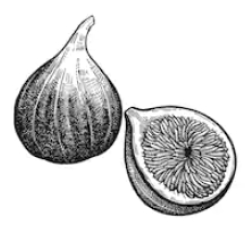
\includegraphics[width=1in,height=1.25in,clip,keepaspectratio]{fig1}}]{Michael Shell}
Use $\backslash${\tt{begin\{IEEEbiography\}}} and then for the 1st argument use $\backslash${\tt{includegraphics}} to declare and link the author photo.
Use the author name as the 3rd argument followed by the biography text.
\end{IEEEbiography}

\vspace{11pt}

\bf{If you will not include a photo:}\vspace{-33pt}
\begin{IEEEbiographynophoto}{John Doe}
Use $\backslash${\tt{begin\{IEEEbiographynophoto\}}} and the author name as the argument followed by the biography text.
\end{IEEEbiographynophoto}




\vfill


\end{document}
